\documentclass{beamer}
%               \usefonttheme{professionalfonts}
%               \usefonttheme[onlysmall]{structureitalicserif}
    \usefonttheme[frametitle]{structuresmallcapsserif}
%    \usetheme{Boadilla}
    \usetheme{Madrid}
    \useoutertheme{progressbar}
        \usecolortheme[]{seahorse}
%       \usecolortheme[]{beetle}
%       \usecolortheme[]{albatross}
%       \usecolortheme[]{wolverine}
%       \usecolortheme[]{crane}
%       \usecolortheme[]{sidebartab}
%       \usecolortheme[]{whale}
%       \usecolortheme[]{rose}
%       \usecolortheme[]{dolphin}
    \useinnertheme{rounded}    % circles, inmargin, rectangles, rounded
%        \newcommand{\includeoptional}{false}
    \newcommand{\includeoptional}{true}
    \setbeamertemplate{headline}{}
    \setbeamertemplate{navigation symbols}[vertical]
    \setbeamertemplate{blocks}[rounded][shadow=false]
%               \setbeamertemplate{frametitle}{}
%               \setbeamertemplate{footline}{}
%               \setbeamersize{text margin right=1cm} % erzeugt einen Randabstand
    \setbeamercovered{transparent}
%\setbeameroption{hide notes} 
\mode<handout>{
  \usetheme{Pittsburgh}
  \usecolortheme[]{default}
%  \usecolortheme{albatross}
%  \usecolortheme{beaver}
%  \usecolortheme{beetle}
  \usecolortheme{crane}
%  \usecolortheme{dolphin}
%  \usecolortheme{dove}
%  \usecolortheme{fly}
%  \usecolortheme{lily}
%  \usecolortheme{orchid}
%  \usecolortheme{rose}
%  \usecolortheme{seagull}
%  \usecolortheme{seahorse}
%  \usecolortheme{whale}
%  \usecolortheme{wolverine}
		\useinnertheme{progressbar}
%		\setbeamertemplate{headline}{}
		\setbeamertemplate{footline}{}
}
%\listfiles
%\documentclass[a4paper,10pt,xcolor=pdftex,dvipsnames,table]{beamer}
%\mode<presentation>{
%%		\usefonttheme{professionalfonts}
%%		\usefonttheme[onlysmall]{structureitalicserif}
%		\usefonttheme[frametitle]{structuresmallcapsserif}
%%		\usetheme{Boadilla}
%		\usetheme{Madrid}
%		\useoutertheme{progressbar}
%		\usecolortheme[]{seahorse}
%%		\usecolortheme[]{crane}
%%		\usecolortheme[]{sidebartab}
%%		\usecolortheme[]{whale}
%%		\usecolortheme[]{rose}
%        \useinnertheme{rounded}    % circles, inmargin, rectangles, rounded
%        \newcommand{\includeoptional}{false}
%%        \newcommand{\includeoptional}{true}
%		\setbeamertemplate{headline}{}
%        \setbeamertemplate{navigation symbols}[vertical]
%        \setbeamertemplate{blocks}[rounded][shadow=false]
%%		\setbeamertemplate{frametitle}{}
%%		\setbeamertemplate{footline}{}
%%		\setbeamersize{text margin right=1cm} % erzeugt einen Randabstand
%        \setbeamercovered{transparent}
%}
%
\usepackage{pgfpages}
\usepackage{color, german, graphicx}
\usepackage{eurosym}
\usepackage{fancyvrb} % use \begin{frame}[fragile] !
\usepackage{xmpmulti}
\selectlanguage{english}
\usepackage{pslatex}
\usepackage{ulem}
\usepackage[absolute,overlay]{textpos}
\usepackage{ifthen} 
\usepackage{hyperref}
\usepackage{ragged2e}
\usepackage[style=authoryear]{biblatex}
%\usepackage{listings}
\usepackage{tikz}
\usepackage{tabu}
\usetikzlibrary{chains, shapes.misc}
%\usetikzlibrary{chains, shapes.misc, shapes.geometric, positioning}
\tikzset{
compartment/.style={ circle, minimum size=10mm, very thick, draw=brown!70!black!50, top color=white, bottom color=brown!70!black!70, font=\itshape },
elm/.style={ rectangle, minimum size=6mm, thick, draw=yellow!90!red!40, top color=white, bottom color=yellow!90!red!40, font=\ttfamily },
protein/.style={ rounded rectangle, minimum size=10mm, thick, draw=blue!50!black!50, top color=white, bottom color=blue!70!black!50, font=\itshape },
connection/.style={ very thick };
arrow/.style={ thick };
}
\hypersetup{%
    colorlinks=true, linktocpage=true, pdfstartpage=1, pdfstartview=FitV,pdfpagelayout=TwoPageRight,%
    breaklinks=true, pdfpagemode=UseNone, pageanchor=true, pdfpagemode=UseOutlines,%
    plainpages=false, bookmarksnumbered, bookmarksopen=true, bookmarksopenlevel=2,%
    hypertexnames=true, pdfhighlight=/O, urlcolor=footersymbolcolor, %
    pdftitle={Short Linear Motifs},%
    pdfauthor={Holger Dinkel},%
    pdfsubject={Short Linear Motif Resources},%
    pdfkeywords={Short Linear Motif},%
    pdfcreator={pdfLaTeX},%
    pdfproducer={LaTeX}%
}

%\usetikzlibrary{graph}
\usepackage{setspace}
%\usepackage{movie15}
\usepackage{fancyvrb}
\DefineShortVerb[commandchars=\\\{\}]{\|}
%\DefineVerbatimEnvironment{Highlighting}{Verbatim}{commandchars=\\\{\}}
% Add ',fontsize=\small' for more characters per line
%\newenvironment{Shaded}{}{}
\newcommand{\PROT}[1]{\alert{\textsc{#1}}}
\renewcommand\mathfamilydefault{\ttdefault}
%
\newcommand{\hogsboxtop}[2]{
\begin{minipage}[t]{.99\textwidth}   
\begin{exampleblock}{#1}
  #2
  \end{exampleblock}
\end{minipage}}
\newcommand{\hogsboxmid}[2]{
\begin{minipage}[t]{.95\textwidth}   
\begin{exampleblock}{#1}
  #2
  \end{exampleblock}
\end{minipage}}
\newcommand{\hogsboxbot}[2]{
\begin{minipage}[t]{.91\textwidth}   
\begin{exampleblock}{#1}
  #2
  \end{exampleblock}
\end{minipage}}
%
\newcommand\Paper[3]{%
\begin{textblock*}{.98\textwidth}(5pt,.98\textheight)%
%\begin{textblock*}{.98\textwidth}(5pt,.93\textheight)%
 \begin{spacing}{.5} 
{\sc\scriptsize \textsl{``\raggedright #1''};
{\tiny #2; (#3)}}
\end{spacing}
\end{textblock*}}

\bibliography{references}

% Set the headline of each frame to subsection:
% \addtobeamertemplate{frametitle}{
%    \let\insertframetitle\insertsubsectionhead}{}
% \makeatletter
%   \CheckCommand*\beamer@checkframetitle{\@ifnextchar\bgroup\beamer@inlineframetitle{}}
%   \renewcommand*\beamer@checkframetitle{\global\let\beamer@frametitle\relax\@ifnextchar\bgroup\beamer@inlineframetitle{}}
% \makeatother

%\setbeameroption{show notes on second screen=right}
%
\begin{document}

\date{EMBO Practical Course ``Computational analysis of protein-protein interactions -- From sequences to networks''}
\title{Short Linear Motifs}
\subtitle{}
\author{Holger Dinkel}

\newcommand{\optional}[1]{\ifthenelse{\equal{\includeoptional}{true}}{#1}{---}}
%
{
\setbeamertemplate{frametitle}{}
\setbeamertemplate{framesubtitle}{}
\setbeamertemplate{navigation symbols}{}
\setbeamertemplate{headline}{}
\begin{frame}[plain]
\note{}
    \titlepage
\end{frame}
%
%\begin{frame}[plain]
%\note{First: Introduction to Short Linear Motifs\\
%    Then, The ELM Resource\\
%    Followed by a monologue about data annotation in general and for the ELM DB in particular.\\}
%    \tableofcontents[sections]
%\end{frame}
}

\section{Short Linear Motifs}

\subsection{Importance of Short Linear Motifs}
\begin{frame}\frametitle{Importance of Short Linear Motifs}
\note{ I'd like to start with this 3d illustration of an interaction between CDK2 \& CyclinA\\
It nicely illustrates an interaction between two globular domains, which still is what most people have in mind when thinking about protein-protein interactions\\
However this example is nice because it also shows another type of interaction: Globular - IDR\\
And it also serves as a demonstration of a third kind of interaction: Globular - motif (which is what I'm most interested in)\\
explain/mention \textbf{functional site}
}
        \only<1|handout:0>{\optional{\includegraphics[width=.95\textwidth]{images/globular_domain_linear_motif1.png}}}%
        \only<2|handout:0>{\optional{\includegraphics[width=.95\textwidth]{images/globular_domain_linear_motif2.png}}}%
        \only<3|handout:0>{\optional{\includegraphics[width=.95\textwidth]{images/globular_domain_linear_motif3.png}}}%
        \only<4|handout:1>{\optional{\includegraphics[width=.95\textwidth]{images/globular_domain_linear_motif4.png}}}%
\end{frame}

\begin{frame}[t]\frametitle{Attributes of Short Linear Motifs}
    \note{
    Linear motifs are \textbf{small} (hence the name Short Linear Motifs)\\
    A couple of years ago we've performed a survey and wrote review about the attributes of short linear motifs.\\
        \begin{itemize}
            \item<1-> are small.
            \item<2-> have few defined positions.
            \item<3-> mediate transient, low affinity interactions.
        \end{itemize}
    }%
    \vspace{-4mm}%
    \begin{block}{Linear Motifs}
        \begin{itemize}
            \item<1-> are small.
            \item<2-> have few defined positions.
            \item<3-> mediate transient, low affinity interactions.
        \end{itemize}
    \end{block}%
    \vspace{-4mm}%
    \begin{center}
        \only<1|handout:0>{\includegraphics[height=.55\textheight]{images/attributes_length.png}}%
        \only<2|handout:0>{\includegraphics[height=.55\textheight]{images/attributes_definedPos.png}}%
        \only<3|handout:1>{\includegraphics[height=.60\textheight]{images/plot_interaction_instances_affinities_vs_length.png}}%
        %    \optional{\includegraphics[width=.95\textwidth]{images/Versatility_in_SLiM_recognition_by_SLiM-binding_domains.pdf}}
    \end{center}
\only<1-2>{\Paper{Attributes of short linear motifs}{Davey, van~Roey, Weatheritt, Toedt, Uyar, Altenberg, Budd, Diella, Dinkel \& Gibson}{Mol Biosyst. 2011}}
\end{frame}

\begin{frame}\frametitle{Prevalence of Short Linear Motifs}
    \begin{block}{Domain frequencies from Pfam (human proteome):}
    \begin{tabu} to \linewidth {ccc}%
    Domain Family & Frequency & Pattern of recognized motif\\%
    & [Domains / Proteins] & \\\hline%
    PDZ & 573 / 342 & $[ST]x[ACVILF]_{−-COOH}$ \\
    SH3 & 451 / 382 & $PxxP$ \\
    SH2 & 237 / 219 & $_{P}Yxx[IV]$ \\
    WW & 151 / 103 & $PPxY$ \\
    PTB & 142 / 133 & $NPx_{p}Y$ \\
    \end{tabu}
    \end{block}
\end{frame}

\begin{frame}\frametitle{Importance of Short Linear Motifs: Viruses}%
    \note<1>{
    Short Linear Motifs are relevant to almost any aspect of cell regulation\\
    Instead of trying to convince you using the usual suspects (Disease, Cancer), I'll try to use just one slide on Viruses:
    Because Viruses are restricted in (genome) size, they abuse (short linear) motifs to mess with the host's cellular machinery,
    outcompeting (in affinity) cellular motif counterparts.\\
    From Viral entry to Egress and almost any step in between, we know many motifs that different viruses abuse.\\
    Need proteins delivered to certain locations? Use the cell's transport system!\\
    Need proteins synthesized? Arrest the cell in the proper cell cycle state!}
    \vspace{-2mm}%
    \begin{center}
        \optional{\includegraphics[height=.8\textheight]{images/davey_fig2.png}}%
    \end{center}
    \Paper{How viruses hijack cell regulation}{Davey, Trav\'{e} \& Gibson}{TiBS 2010}%
\end{frame}

\begin{frame}[t]\frametitle{Importance of Short Linear Motifs: Diseases}
        \note{The Bacillus-produced anthrax toxin LF (lethal factor), a
        protease, cleaves the N-terminal MAPK docking motif of several MAPK kinases
        (MAPKK).402 The catalytic domain of LF appears to have evolved specificity to
        target MAPK docking motifs, allowing B. anthracis to inhibit signaling through
        the MAPK pathways by disrupting MAPKK binding to MAPK and thereby block MAPKK
        phosphorylation of MAPK}%
%        \vspace{-1.25em}%
        \vfill See also \url{http://elm.eu.org/infos/diseases.html}%
        \only<1|handout:0>{\hogsboxtop{Liddle's-Syndrome: WW-Interaction motif}{%
        has been implicated with autosomal dominant activating mutations in the WW interaction motif in the $\beta${}- and
        $\gamma${}-subunits of the epithelial sodium channel \PROT{ENaC}. These mutations abrogate the binding to the
        ubiquitin ligase \PROT{NEDD4-2}, %thereby inhibiting channel degradation and prolonging the half-life of \PROT{ENaC}, 
        ultimately resulting in increased Na$^+$ reabsorption, plasma volume extension and hypertension.
        }}%
        %  \vspace{1em}%
        \only<2|handout:0>{\hogsboxtop{Bacillus anthracis ``lethal factor''}{%
        The protein \PROT{LEF\_BACAN} is a metalloprotease that specifically
        targets mitogen-activated protein kinase kinases (MKKs).
        which are important regulators of signal transduction
        as they phosphorylate and thus activate specific MAPKs (such as ERK1, ERK2, p38
        or JNK). Bacillus anthracis' ``lethal factor'' cleaves its MKK substrates within
        or close to the MAPK docking sites, thus effectively preventing the MKK to dock to its MAPK.
        }}%
%        \only<2|handout:0>{\hogsboxtop{Usher's-Syndrome: PDZ-domain/-motif}{%
%        is the most frequent cause of hereditary deaf-blindness in humans, affecting one child in
%        25\,000.  This disease can be caused by mutations in either PDZ domains in \PROT{Harmonin} or the corresponding PDZ interaction motifs in
%        \PROT{SANS} protein.
%        }}%
    \end{frame}

\begin{frame}[t]\frametitle{Importance of Short Linear Motifs: Cancer}
%        \vspace{-1.25em}%
        \only<1|handout:1>{\hogsboxtop{$\beta{}$--Catenin}{%
%        \\
        \begin{minipage}[\textheight]{\textwidth}
            \begin{columns}[T]
                \begin{column}{0.3\textwidth}
                    \vspace{2mm}\optional{\includegraphics[height=.35\textheight]{images/b-catenin_TrCP1.png}
                \end{column}
                \begin{column}{0.7\textwidth}
                    \vspace{2mm}The most recurrently mutated experimentally validated SLiM in the COSMIC DB
                    is the conserved proteasomal degradation motif in the highly disordered N-terminal
                    region of $\beta${}-Catenin which mediates binding to the WD40 repeat domain of the
                    $\beta${}-TRCP subunit of the SCF-betaTRCP E3 ubiquitin ligase complex. (more
                    than 1700 mutation entries for this motif derived from 1692 unique samples
                    based on 256 different publications)
                \end{column}
            \end{columns}
        \end{minipage}
        }%
        }}%
        \\ \vspace{0.5em}%
        \only<1|handout:1>{\Paper{Proteome-wide analysis of human disease mutations in short linear motifs: neglected players in cancer?}{Uyar, Weatheritt, Dinkel, Davey \& Gibson}{Mol. Biosyst.; 2014}}
    \end{frame}

\begin{frame}\frametitle{Importance of Short Linear Motifs: P53}
    \note{ Everybody's pet protein: P53! Arguably one of the most important proteins in the cell?! Full of linear motifs! \\DNA-binding \& tetrametization domain in the middle, Rest=motifs.\\
    DNA, 53BP1, gcn5, p53-tetrametization domain, set9, cyclinA, sirtuin, CBP bromo domain, s100ββ, sv40 Large T antigen, 53BP2, PH, MDM2, rpa70. }
    \vspace{-2mm}%
    \begin{center}
        \optional{\includegraphics[height=.85\textheight]{images/uversky_dunker.png}}%
    \end{center}
    \Paper{Understanding protein non-folding}{Uversky \& Dunker}{Biochimica et Biophysica Acta 2010}%
\end{frame}


\begin{frame}\frametitle{Motifs in external proteins}
    \note{Allegra’s RGD motif in solved structures is a good illustration of how 
    extracellular motifs tend to be in loops of folded regions, IUP being much rarer 
    in extracellular proteins (exceptions like mucins, collagens). Also two of the examples are parasite uses.
    %
    Solved structures of three different RGD--containing proteins. RGD motifs are
    shown as orange sticks. The occurrence of identical motifs on completely
    unrelated scaffolds supports the hypothesis they represent convergent evolution
    events. Bottom left: Human Del-1 EGF2 domain. The RGD motif forms a type II'
    beta turn at the tip of a long loop, dubbed the RGD finger, which is critical
    for integrin binding; PDB: 4D90; bottom middle: Secreted aspartic proteinase
    from C. albicans; PDB 4QZX; bottom right: RGD-containing
    host-selective toxin Ptr ToxA from P. tritici-repentis; PDB: 1ZLD. }%

    SLiMs play even a role in extracellular proteins as highlighted by these solved structures of three different RGD--containing proteins. 
    (The occurrence of identical motifs on completely unrelated scaffolds supports the hypothesis they represent convergent evolution events).\\
    \smaller{(Note how these extracellular motifs are located in loops of folded regions.)}
    \begin{center}
        \visible<+->{\optional{\includegraphics[height=.55\textheight]{images/Uyar_Via_RGD_1.png}}}
        \visible<+->{\optional{\includegraphics[height=.55\textheight]{images/Uyar_Via_RGD_2.png}}}
        \visible<+->{\optional{\includegraphics[height=.55\textheight]{images/Uyar_Via_RGD_3.png}}}
    \end{center}
    \Paper{How pathogens use linear motifs to perturb host cell networks}{Via et~al.}{Trends Biochem Sci. 2015}
\end{frame}

\subsection{Classification of Motifs}
\begin{frame}\frametitle{Classification of Motifs}
    \optional{\includegraphics[width=.95\textwidth]{images/motif_classification.png}}
\end{frame}

%\subsection{Modification Sites}
\begin{frame}[t]\frametitle{Motif Classes: Modification Sites}
    \note{Phosphorylation, Myristoylation, Glycosylation,... \\
    We know hundreds of thousands of these! In fact there exists so many that databases exist that collect instances of these...\\
    Sites of post-translational modification by mediate binding to the active site of a modifying enzyme.
    }
    \vspace{-5mm}
    \begin{columns}[T]
        \begin{column}{.49\textwidth}
            \begin{alertblock}{Description:}
                Modification Motifs mediate specific binding to the active site of a modifying enzyme to allow subsequent catalytic post-translational
                modification of the target site.
            \end{alertblock}
            \end{column}
            \begin{column}{.49\textwidth}
                \begin{exampleblock}{Example:}
                    \begin{description}[RegEx]
                        \item[Name] MOD\_CDK\_1
                        \item[RegEx] {\tt $ xxx([ST])Px[KR]$}
                    \end{description}
                \end{exampleblock}
            \end{column}
        \end{columns}
    \begin{center}
    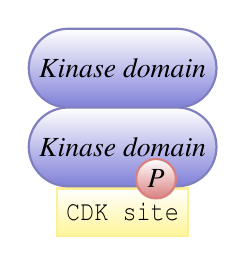
\begin{tikzpicture}[node distance=5mm]
        \node (pmotif) [elm] {CDK site};
        \visible<1,4|handout:0>{\node (kdomain) [protein, above=of pmotif, yshift=5mm, minimum size=10mm] {Kinase domain};}
        \visible<2,3|handout:1>{\node (kdomain2) [protein, above=of pmotif, yshift=-5mm, minimum size=10mm] {Kinase domain};}
        \visible<3->{\node (phospho) [protein, draw=red!70!black!50, bottom color=red!70!black!50, minimum size=5mm, above right of=pmotif, node distance=6mm] {P};}
    \end{tikzpicture}
    \end{center}
%    \Paper{Phospho.ELM: a database of phosphorylation sites -- update 2011}{Dinkel, Chica, Via, Gould, Jensen, Gibson \& Diella}{ Nucleic Acids Res. 2011}
\end{frame}

%\subsection{Docking Motifs}
\begin{frame}[t]\frametitle{Motif Classes: Docking Motifs}
    \note{ Related to Modification sites are Docking Motifs, like DOC\_CYCLIN\_1 mentioned before\\
           \textbf{recruit} enzymes usually via a surface that is distinct from the enzyme's active site.
    }
    \vspace{-5mm}
    \begin{columns}[T]
        \begin{column}{.49\textwidth}
            \begin{alertblock}{Description:}
                Docking motifs recruit enzymes via a surface that is distinct from the active site.
                \end{alertblock}
            \end{column}
            \begin{column}{.49\textwidth}
                \begin{exampleblock}{Example:}
                    \begin{description}[RegEx]
                        \item[Name] DOC\_CYCLIN\_1
                        \item[RegEx] $ [RK]xLx\{0,1\}[LFY]$
%                       Docking site in substrates and inhibitors of cyclin-CDK complexes. 
                    \end{description}
                \end{exampleblock}
            \end{column}
        \end{columns}
    \begin{center}
    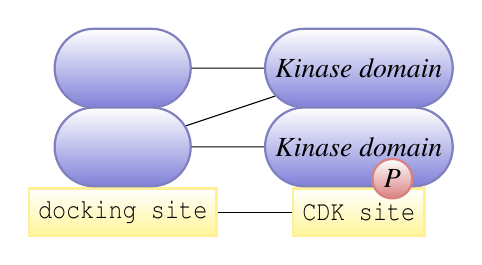
\begin{tikzpicture}[node distance=5mm]
        \node (pmotif) [elm] {CDK site};
        \node (dmotif) [elm,left of=pmotif, node distance=30mm] {docking site};
        \visible<1,2,5|handout:1>{\node (kdomain) [protein, above=of pmotif, yshift=5mm, minimum size=10mm] {Kinase domain};}
        \visible<3,4|handout:0>{\node (kdomain2) [protein, above=of pmotif, yshift=-5mm, minimum size=10mm] {Kinase domain};}
        \visible<1,5|handout:0>{\node (ddomain) [protein, minimum size=10mm, left of=kdomain, node distance=30mm] {~~~~~~~~~~~~~~~~~~};}
        \visible<2,3,4|handout:1>{\node (ddomain2) [protein, minimum size=10mm, left of=kdomain2, node distance=30mm] {~~~~~~~~~~~~~~~~~~};}
        \visible<4-|handout:0>{\node (phospho) [protein, draw=red!70!black!50, bottom color=red!70!black!50, minimum size=5mm, above right of=pmotif, node distance=6mm] {P};}
        \path[connection] (pmotif) edge[-] (dmotif);
        \visible<1,5|handout:0>{\path[connection] (kdomain) edge[-] (ddomain);}
        \visible<2|handout:1>{\path[connection] (kdomain) edge[-] (ddomain2);}
        \visible<3-4|handout:0>{\path[connection] (kdomain2) edge[-] (ddomain2);}
    \end{tikzpicture}
    \end{center}
\end{frame}

%\subsection{Cleavage Motifs}
\begin{frame}[t]\frametitle{Motif Classes: Cleavage Motifs}
    \note{
            Recognized by \texbf{Proteases}\\
            Proteolytically process the protein into smaller polypeptides by hydrolysing specific peptide bonds 
    }
    \vspace{-5mm}
    \begin{columns}[T]
        \begin{column}{.49\textwidth}
            \begin{alertblock}{Description:}
                 Proteolytic processing of proteins into smaller polypeptides by protease-catalyzed hydrolysis of specific peptide bonds 
                \end{alertblock}
            \end{column}
            \begin{column}{.49\textwidth}
                \begin{exampleblock}{Example:}
                    \begin{description}[RegEx]
                        \item[Name] CLV\_Separin\_Metazoa
                        \item[RegEx] $ E[IMPVL][MLVP]Rx$
                    \end{description}
                \end{exampleblock}
            \end{column}
        \end{columns}
    \begin{center}
    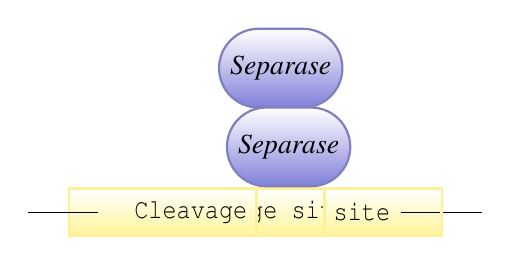
\begin{tikzpicture}[node distance=5mm]
        \visible<1,2|handout:0>{\node (motif) [elm] {~~~~Cleavage site~~~~};}
        \visible<3,4|handout:1>{\node (motif1) [elm, right of=motif, xshift=-16mm] {~~~~Cleavage};}
        \visible<3,4|handout:1>{\node (motif2) [elm, right of=motif, xshift=12mm] {site~~~~};}
        \visible<1,4|handout:0>{\node (cdomain)  [protein, above=of motif, yshift=5mm,  xshift=4mm, minimum size=10mm] {Separase};}
        \visible<2,3|handout:1>{\node (cdomain2) [protein, above=of motif, yshift=-5mm, xshift=5mm, minimum size=10mm] {Separase};}
        \visible<1,2|handout:0>{\draw (motif.west) -- ++(-0.5,0);
        \draw (motif.east) -- ++(0.5,0);}
        \visible<3,4|handout:1>{\draw (motif1.west) -- ++(-0.5,0);
        \draw (motif2.east) -- ++(0.5,0);}
    \end{tikzpicture}
    \end{center}
\end{frame}

%\subsection{Degradation Motifs}
\begin{frame}[t]\frametitle{Motif Classes: Degradation Motifs}
    \note{ 
    \textbf{Degrons}Selective degradation of specific proteins by ubiquitin-mediated proteolysis plays an important role in controlling a wide variety 
    of cellular processes, such as the cell cycle and apoptosis and allows proteins to exhibit widely differing half-lives, ranging from a few minutes to several days\\
    }
    \vspace{-5mm}
    \begin{columns}[T]
        \begin{column}{.49\textwidth}
            \begin{alertblock}{Description:}
                    Degradation motifs (Degrons) recognized by E3 Ubiquitin Ligase complexes priming proteins for degradation, regulating protein half-life.
                \end{alertblock}
            \end{column}
            \begin{column}{.49\textwidth}
                \begin{exampleblock}{Example:}
                    \begin{description}[RegEx]
                        \item[Name]DEG\_SCF\_TRCP1\_1\\
                        \item[RegEx] $ D(S)Gxx([ST])$\\
                        %            \item[Description] Phospho-dependent degron recognized by the FBXW7 subunit of the SCF ubiquitin ligase.
                    \end{description}
                \end{exampleblock}
            \end{column}
        \end{columns}
    \begin{center}
    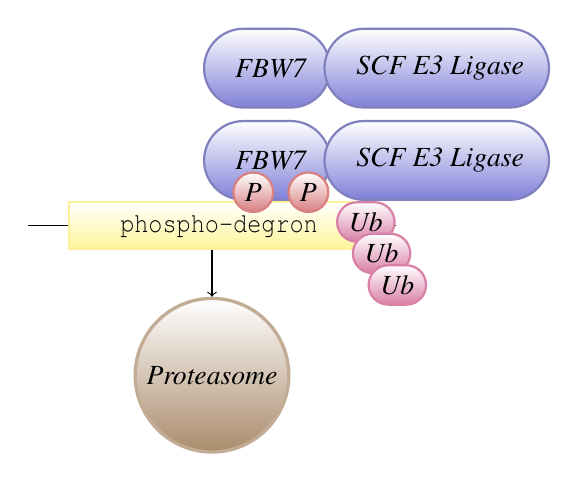
\begin{tikzpicture}[node distance=5mm]
        \node (pmotif) [elm] {~~~phospho-degron~~~};
        \draw (pmotif.west) -- ++(-0.5,0);
        \draw (pmotif.east) -- ++(0.5,0);
        \visible<1,4-|handout:0>{
            \node (kdomain) [protein, node distance=20mm, above of=pmotif, xshift=7mm, minimum size=10mm] {~~~FBW7~~~};
            \node (ligase) [protein, node distance=-1mm, right=of kdomain, minimum size=10mm] {~~~SCF~E3 Ligase~~~};
            }
        \visible<2-3|handout:1>{
            \node (kdomain2) [protein, above=of pmotif, xshift=7mm, yshift=-5mm, minimum size=10mm] {~~~FBW7~~~};
            \node (ligase2) [protein, node distance=-1mm, right=of kdomain2, minimum size=10mm] {~~~SCF~E3 Ligase~~~};
            }
        \visible<4-|handout:1>{\node (proteasome) [compartment, below of=pmotif, node distance=19mm] {Proteasome};}
        \visible<1-|handout:1>{
        \node (phospho) [protein, draw=red!70!black!50, bottom color=red!70!black!50, minimum size=5mm, above right of=pmotif, node distance=6mm, xshift=1mm] {P};
        \node (phospho) [protein, draw=red!70!black!50, bottom color=red!70!black!50, minimum size=5mm, above right of=pmotif, node distance=6mm, xshift=8mm] {P};
        }
        \visible<3-|handout:1>{
        \node (ubiquitin) [protein, draw=red!70!blue!50, bottom color=red!70!blue!50, minimum size=5mm, below right of=pmotif, xshift=16mm, yshift=4mm] {Ub};
        \node (ubiquitin) [protein, draw=red!70!blue!50, bottom color=red!70!blue!50, minimum size=5mm, below right of=pmotif, xshift=18mm, yshift=0mm] {Ub};
        \node (ubiquitin) [protein, draw=red!70!blue!50, bottom color=red!70!blue!50, minimum size=5mm, below right of=pmotif, xshift=20mm, yshift=-4mm] {Ub};
        }
        \visible<4-|handout:1>{ \path[] (pmotif.south) edge[->] (proteasome); }
    \end{tikzpicture}
    \end{center}
\end{frame}

%\subsection{Targeting/Anchoring Motifs}
\begin{frame}[t]\frametitle{Motif Classes: Targeting/Anchoring Motifs}
    \note{
        \structure{Targeting} motifs usually bind to transport protein/vehicle that relocalizes it to a particular sub-cellular location.\\
        Well known example: \textbf{NLS}\\
        \structure{Anchoring} motifs usually retain the motif-containing protein in a particular location (eg. \textbf{membrane}).
    }
    \vspace{-5mm}
    \begin{columns}[T]
        \begin{column}{.49\textwidth}
            \begin{alertblock}{Description:}
        \structure{Targeting} motifs allow a protein to bind to the transport machinery that relocalizes it to a particular sub-cellular location.\\
        \structure{Anchoring} motifs are recognized by biomolecules specific to a sub-cellular location and thereby retain the motif-containing protein at that location.
%        Nuclear localization signal (NLS); motif recognized by the Armadillo repeats of Importin subunit $\alpha$ for import into the nucleus.
                \end{alertblock}
            \end{column}
            \begin{column}{.50\textwidth}
                \begin{exampleblock}{Example:}
                    \begin{description}[RegEx]
                        \item[Name] TRG\_NLS\_MonoCore\_2%
                        \item[RegEx]{\footnotesize$[~\hat{}DE](K[RK]\text{\textbar}RK)[KRP][KR][~\hat{}DE]$}%
                    \end{description}
                \end{exampleblock}
            \end{column}
        \end{columns}
    \begin{center}
    \vspace{-5mm}\begin{tikzpicture}
        \node (motif) [elm] {NLS};
        \node (hiddennode) [right of=motif, xshift=7mm, yshift=5mm] {};
        \visible<1|handout:0>{\node (domain) [protein, above of=motif, node distance=17mm] {Importin $\alpha$};}
        \visible<2-|handout:1>{\node (domain2) [protein,above of=motif, node distance=8mm] {Importin $\alpha$};}
        \visible<3-|handout:1>{\node (nucleus) [compartment, right of=motif, yshift=14mm, node distance=50mm, minimum size=30mm] {Nucleus};}
        %\visible<1>{\path[arrow] (domain) edge[->] (motif);}
        %\draw (domain) -- ++(2,0) -- (motif);
        \visible<3-|handout:1>{\path[] (motif.east) edge[--] (hiddennode.west);
        \path[] (domain2) edge[--] (hiddennode.west);
        \path[] (hiddennode.west) edge[->] (nucleus);}
        \visible<1-|handout:1>{\draw (motif.west) -- ++(-0.5,0);
        \draw (motif.east) -- ++(0.5,0);}
    \end{tikzpicture}
    \end{center}
\end{frame}

% \begin{frame}[t]
%     %    \optional{\includegraphics[width=.95\textwidth]{images/Functionality_of_ligand_motifs.pdf}}
%     \begin{columns}[T]
%         \begin{column}{.49\textwidth}
%     \begin{block}{Motif Class}%{Short Linear Motif categories:}
%         %        \begin{description}[Ligand Binding]
%             %            \item<1->[Anchoring] PIP Box; motif recognized by Proliferating Cell Nuclear Antigen (PCNA) for association of proteins involved in DNA replication, DNA repair and cell cycle control with the DNA replication fork.
%             %            \item<2->[Cleavage] Separase cleavage motif.
%             %            \item<3->[Docking] Docking site in substrates and inhibitors of cyclin-CDK complexes.
%             %            \item<4->[Degron] Phospho-dependent degron recognized by the FBXW7 subunit of the SCF ubiquitin ligase.
%             %            \item<5->[Ligand Binding] Src Homology 3 (SH3) domains binding motif.
%             %            \item<6->[Modification] Phosphorylation site modified by CDK.
%             %            \item<7->[Trafficking] Nuclear localization signal (NLS); motif recognized by the Armadillo repeats of Importin subunit $\alpha$ for import into the nucleus.
%                 %        \end{description}
%         \begin{itemize}[<+->]
%             \item Anchoring
%             \item Cleavage
%             \item Docking
%             \item Degron
% %            \item Ligand Binding
%             \item Modification
%             \item Trafficking
%         \end{itemize}
%     \end{block}
%         \end{column}
%         \begin{column}{.49\textwidth}
%     \begin{exampleblock}{Example:}
%             \only<1>{\structure{LIG\_PCNA\_PIPBox\_1}\\
%                 $ Qxx\phixx[HFM][FMY] $\\
%                 PIP Box; motif recognized by Proliferating Cell Nuclear Antigen (PCNA) for association of proteins involved in DNA replication, DNA repair and cell cycle control with the DNA replication fork. }
%             \only<2>{\structure{CLV\_Separin\_Metazoa}\\
%                 $ E[IMPVL][MLVP]Rx$\\
%                 Separase cleavage motif. }
%             \only<3>{\structure{DOC\_CYCLIN\_1}\\
%                 $ [RK]xLx\{0,1\}[LFY]$\\
%                 Docking site in substrates and inhibitors of cyclin-CDK complexes. }
%             \only<4>{\structure{DEG\_SCF\_TRCP1\_1}\\
%                 $ D(S)Gxx([ST])$\\
%                 Phospho-dependent degron recognized by the FBXW7 subunit of the SCF ubiquitin ligase. }
%             \only<5>{\structure{LIG\_SH3\_2}\\
%                 $ PxxPx[KR]$\\
%                 Src Homology 3 (SH3) domains binding motif. }
%             \only<6>{\structure{MOD\_CDK\_1}\\
%                 $  xxx([ST])Px[KR]$\\
%                 Phosphorylation site modified by CDK. }
%             \only<7>{\structure{TRG\_NLS\_MonoCore\_2}\\
%                 $ [~\hat{}DE]((K[RK])\|(RK))[KRP][KR][~\hat{}DE]$\\
%                 Nuclear localization signal (NLS); motif recognized by the Armadillo repeats of Importin subunit $\alpha$ for import into the nucleus. }
%     \end{exampleblock}
%         \end{column}
%     \end{columns}
% \end{frame}

\begin{frame}[t]\frametitle{Motif Classes: Targeting/Anchoring Motifs}
    \note{This schema illustrates the most important cellular compartments, and how motifs mediate trafficking to/from these\\
Note also how anchoring motifs retain proteins in certain localizations. }
    \begin{center}
        \only<1>{\vspace{-5mm}\optional{\includegraphics[height=.85\textheight]{images/Functionality_of_targeting_motifs_trans.png}}}%
        \only<2|handout:1>{\vspace{-5mm}\optional{\includegraphics[height=.85\textheight]{images/Functionality_of_targeting_motifs.png}}}%
    \end{center}
    \Paper{Short linear motifs: Ubiquitous and functionally diverse protein interaction modules directing cell regulation}{van~Roey, Uyar, Weatheritt, Dinkel, Seiler, Budd, Gibson \& Davey}{Chem. Reviews; 2014}
\end{frame}

%\section{The Eukaryotic Linear Motif Resource}
%{
%\setbeamertemplate{frametitle}{}
%\setbeamertemplate{framesubtitle}{}
%\setbeamertemplate{navigation symbols}{}
%\setbeamertemplate{headline}{}
%\begin{frame}[plain]
%\note{With this I'd like to switch to the next section, introducting the ELM resource.}
%    \tableofcontents[currentsection]
%\end{frame}
%}
%

\begin{frame}\frametitle{Visualizing Motif-Mediated Interactions}
    \note{
    By making this data available via a \tebtbf{RESTful interface},
    With this kind of information people can go ahead and do all kinds of things.\\\textbf{Matt Rogon}
    }
    \only<1>{\optional{\includegraphics[width=1.1\textwidth]{images/elm_interactions_cys.png}}}
    \only<2>{\optional{\includegraphics[width=.9\textwidth]{images/kegg_pathway_resizedCMYK.pdf}}}
\end{frame}

\subsection{Outlook: The ELM Resource}
\begin{frame}[t]\frametitle{Outlook: The ELM Resource}
    \note{ The Eukaryotic Linear Motif resource is a \structure{database} of over 240 thoroughly annotated motif
        classes with over 2700 annotated instances. \\
        It is also a \structure{prediction tool} to find instances of these motif classes in protein sequences. }
    \begin{center}\optional{\includegraphics[width=.8\textwidth]{images/elm_title.png}}\end{center}\\%
    ELM is a \structure{repository} of more than 240 thoroughly annotated motif
    classes with over 2700 annotated instances. \\
    It is also a \structure{prediction tool} to detect these motifs in protein sequences employing different filters to distinguish between \alert{functional}
    and \alert{non-functional} motif instances.\\%
%    \Paper{The eukaryotic linear motif resource ELM: 10 years and counting}{Dinkel, van~Roey, Michael, Davey, Weatheritt, Born, Speck, Kr"uger, Grebnev, Kuba\'{n}, Strumillo, Uyar, Budd, Altenberg, Seiler, Chemes, Glavina, S\'{a}nchez, Diella \& Gibson}{Nucleic~Acids~Res.~2014}
\end{frame}

% \subsection{Switches.ELM}
% \begin{frame}[t]\frametitle{Switches.ELM}
%     \note{adding a sort-of time-vector\\competition switch: CCN-CDK = aforementioned DOC\_Cyclin\_1, overlapping DOC\_PP1\\
% 
%     }
%     \begin{center}
%     \vspace{-5mm}%\optional{\includegraphics[width=.2\textwidth]{images/switches/switches_elm_logo.png}}\\
% %    \framezoom<1|handout:0><1|handout:0>(3.8cm,0.58cm)(3.7cm,2cm)
% %    \framezoom<1|handout:0><2|handout:0>(3.8cm,2.5cm)(3.7cm,2cm)
% %    \framezoom<1|handout:0><2|handout:0>(-0.2cm,0cm)(1.8cm,2.5cm) 
%     \only<1|handout:0>{\vspace{15mm}\optional{\includegraphics[width=.6\textwidth]{images/switches/switches_overview_1_nls.png}}}%
%     \only<2|handout:0>{\vspace{15mm}\optional{\includegraphics[width=.6\textwidth]{images/switches/switches_overview_1_cdk.png}}}%
%     \only<3|handout:0>{\optional{\includegraphics[width=.9\textwidth]{images/switches/switches_overview_1.png}}}%
%     \only<4|handout:0>{\optional{\includegraphics[width=.9\textwidth]{images/switches/switches_overview_2.png}}}%
% %    \only<5|handout:0>{\optional{\includegraphics[width=.9\textwidth]{images/switches/switches_elm_start.png}}\\}
%     \only<5|handout:1>{\optional{\includegraphics[height=.8\textheight]{images/switches/switches_elm_0055.png}}}%
%     \end{center}
%     \only<1-4|handout:0>{\Paper{Motif switches: decision-making in cell regulation.}{van~Roey, Gibson \& Davey}{Curr Opin Struct~Biol.~2012}}
%     \only<5|handout:1>{\Paper{The switches.ELM resource: a compendium of conditional regulatory interaction interfaces.}{van~Roey, Dinkel, Weatheritt, Gibson \& Davey}{Sci. Signal. 2013}}
% %    \optional{\includegraphics[width=.95\textwidth]{images/diagrams/SWTI000339.png}}
% \end{frame}
%
%
\section{Summary} 
\begin{frame}\frametitle{Summary} 
    \begin{block}{Short Linear Motifs}
        \begin{itemize}
        \item small, versatile modules which mediate transient interactions
        \item important regulators of cellular processes.
        \item ``kidnapped'' by viruses
        \item play an important role in diseases
        \item collected in the Eukaryotic Linear Motif Resource (ELM)
        \end{itemize}
    \end{block} 
    % \begin{exampleblock}{The ELM Resource}
    %    \begin{itemize}
    %    \item World's largest freely accessible database of short linear motifs.
    %    \item Providing this service to the scientific community for more than 10 years.
    %    \end{itemize}
    % \end{exampleblock} 
\end{frame}

\appendix

%\begin{frame}[t]\frametitle{Acknowledgments} 
%\note{ All of the Gibson Group, foremost Toby and also Kim: Very much enjoyed working with you.}
%\vspace{-4mm}%
%    \begin{columns}[T]
%        \begin{column}{.4\textwidth}
%            \begin{exampleblock}{Gibson Team}
%                \begin{itemize}
%                    \item Brigitte Altenberg
%                    \item Aidan Budd
%                    \item Norman Davey
%                    \item Francesca Diella
%                    \item \alert{\underline{Toby Gibson}}
%                    \item Vladislava Milchevskaya
%                    \item \alert{\underline{Kim van Roey}}
%                    \item Grischa Toedt
%                    \item Bora Uyar
%                    \item Robert Weatheritt
%                \end{itemize}
%            \end{exampleblock}
%            \begin{exampleblock}{Bio-IT Centers}
%                \begin{itemize}
%                    \item Matt Rogon
%                \end{itemize}
%            \end{exampleblock}
%        \end{column}
%        \begin{column}{.5\textwidth}
%            \begin{alertblock}{More than 70 scientists from all over the world
%                contributing to ELM}
%                \begin{itemize}
%                    \item Annotatation
%                    \item Data submission
%                    \item Code/Algorithm development
%                    \item \ldots{}
%                \end{itemize}
%            \end{alertblock}
%            \begin{block}{Open Source Community}
%                \begin{itemize}
%                    \item Python
%                    \item Django
%                    \item PostgreSQL
%                    \item Linux
%                \end{itemize}
%            \end{block}
%        \end{column}
%    \end{columns}
%\end{frame}

\section{}
\begin{frame}<presentation:1|handout:0>[t]\frametitle{Questions?}
    \note{~}
    \begin{center}
        \optional{\includegraphics[height=.8\textheight]{images/question_moustache.jpg}}
    \end{center}
\end{frame}
%

\end{document}
